\documentclass[conference]{IEEEtran}
\usepackage{amsmath}
\usepackage{graphicx}
\usepackage{algorithm}
\usepackage{algorithmic}
\usepackage{hyperref}
\usepackage{amssymb}

\title{Parallelized All to All Approximate Nearest Neighbors Solution}
\author{\IEEEauthorblockN{Rousomanis Georgios (10703)}
\IEEEauthorblockA{Department of Electrical and Computer Engineering\\
Aristotle University of Thessaloniki\\
Email: rousoman@ece.auth.gr}
}

\begin{document}
\maketitle

\begin{abstract}
This report presents the design and implementation of a parallelized solution to the all-to-all 
approximate nearest neighbors (A2A-ANN) problem, with an emphasis on scalability and computational 
efficiency. While the ultimate objective is to accelerate approximate similarity search in 
high-dimensional spaces where the query and candidate sets are identical ($Q = C$), the current 
work establishes a robust foundation by first solving the generalized exact k-nearest neighbors 
(k-NN) problem for the case where $Q \neq C$. The proposed implementation leverages multi-threaded 
processing and efficient matrix operations to parallelize the distance computation and top-$K$ 
selection stages. We outline the core algorithmic components, discuss strategies for memory-efficient 
execution, and lay the groundwork for extending the approach to approximate search in large-scale datasets.

\end{abstract}

\section{Introduction}
Finding the $K$ nearest neighbors (k-NN) of a point in a dataset is a fundamental operation in a wide 
range of applications, including machine learning, computer vision, information retrieval, and recommendation
systems. In its classical form, the k-NN algorithm identifies, for each query vector, the $K$ closest vectors 
in a reference dataset based on a distance metric—commonly the Euclidean distance.

This report addresses the challenge of scaling the k-NN algorithm to large datasets by parallelizing the 
computation. The ultimate goal is to solve the all-to-all approximate nearest neighbors (A2A-ANN) problem, 
where the query and candidate datasets are identical ($Q = C$), and exactness can be traded off for speed. 
This form of similarity search arises frequently in applications such as clustering, graph construction, 
and manifold learning.

As a foundational step toward the A2A-ANN goal, we begin with a parallelized implementation of the 
generalized exact k-NN problem ($Q \neq C$). This allows us to validate the parallel architecture, distance
computation kernel, and top-$K$ selection strategy in a controlled setting before introducing approximation 
techniques.

Key contributions of this work include:
\begin{itemize}
    \item A parallelized implementation of the exact k-NN algorithm optimized for multi-core CPUs, 
    featuring block-wise processing and thread-level workload balancing.
    \item An extension of the exact framework to an approximate all-to-all nearest neighbors solution 
    using clustering to reduce computational complexity.
    \item A memory-efficient design that adapts dynamically to hardware constraints and minimizes overhead 
    through reuse of pre-allocated buffers.
    \item Comprehensive benchmarking on standard datasets demonstrating significant throughput gains while 
    maintaining acceptable levels of recall.
\end{itemize}

This report focuses on both the algorithmic design and practical implementation aspects, including 
parallelization strategies, memory management techniques, and the trade-offs between accuracy and 
computational efficiency. The remainder of the report is organized as follows: Section II presents 
the parallelized exact k-NN algorithm and its performance benchmarks. Section III details the approximate 
A2A-ANN solution based on clustering and evaluates its scalability and accuracy trade-offs. Finally, 
Section IV concludes with a summary of findings and directions for future work.


\section{Parallelized k-Nearest Neighbors}

The core objective of the algorithm is to identify the $K$ nearest neighbors for each row in a query 
matrix $Q \in \mathbb{R}^{M \times L}$, by comparing it against a reference matrix $C \in \mathbb{R}^{N \times L}$.
Although this report initially assumes $Q \neq C$, the framework is designed to extend seamlessly to the all-to-all
setting where $Q = C$.

To measure similarity between vectors, the squared Euclidean distance is used. This choice simplifies the 
computation as it can be expressed in a form that enables precomputation and vectorized operations:

\[
D = \sqrt{C^2 - 2CQ^\top + {Q^2}^{\top}}
\]
where the square root and the exponentiation are computed element-wise.

\subsection{Parallelization Strategy and Task Management}

To ensure scalability and efficient utilization of computational resources, the algorithm employs multi-threaded 
parallelization based on \texttt{pthreads}, offering fine-grained control over thread management and workload 
distribution. The overall computation is structured around a block-wise processing strategy, where the query 
matrix $Q$ is partitioned into blocks that are dynamically sized to respect the memory constraints of the system. 
Each block is processed independently in parallel before proceeding to the next, ensuring predictable memory usage 
and stable performance across varying hardware configurations.

The principal components of the parallelization pipeline are as follows:

\begin{itemize}
    \item Precomputation of squared norms of all row vectors in $C$, enabling efficient vectorized computation 
    of pairwise distances.
    \item Distribution of each query block's workload across threads, with each thread assigned a contiguous 
    subset of queries to minimize synchronization overhead.
    \item Batched computation of distances between subsets of $Q$ and the full corpus $C$ using optimized matrix 
    multiplication routines (e.g., GEMM from OpenBLAS), which maximizes cache locality and takes advantage of 
    low-level CPU vectorization (SIMD).
    \item Thread synchronization after completion of each query block, ensuring correctness and consistent 
    progression across computational phases.
\end{itemize}

Each thread operates independently within its assigned portion of the query block, following a pipeline 
that includes distance computation, incorporation of precomputed norms, and top-$K$ selection. 
The top-$K$ nearest neighbors are identified using a QuickSelect-based partial selection algorithm, 
which avoids the computationally intensive full sort and achieves expected linear time complexity, 
significantly accelerating the nearest neighbor identification phase.

\subsection{Memory Management Considerations}

Memory management is handled explicitly, with per-thread memory buffers pre-allocated and reused across 
blocks to minimize frequent allocations and deallocations. The size of the query blocks is adaptively 
tuned at runtime based on empirical measurements of available memory and cache performance, ensuring high 
throughput while avoiding memory overcommitment. Additionally, the use of blocked matrix multiplication 
reduces cache misses and optimizes utilization of the CPU’s hierarchical memory.

\subsection{Validation and Robustness}

The correctness of the implementation was validated against Scikit-Learn’s \texttt{NearestNeighbors} module, 
using multiple random datasets and rigorous cross-checking of both distance values and neighbor indices. 
Numerical consistency was ensured through unit testing with controlled seeds and reproducibility of results.

Overall, this design combines low-level threading control, efficient numerical computation, and adaptive memory 
management, establishing a robust and scalable framework for high-performance exact nearest neighbor computation. 
These architectural decisions lay a solid foundation for future integration of approximate search techniques and 
extension to the all-to-all nearest neighbor problem.


\subsection{k-Nearest Neighbors Benchmarks}

We evaluated the performance of the exact k-NN implementation by varying the number of threads used during 
execution. Benchmarks were conducted using the MNIST dataset on a 4-core system running Ubuntu 22.04 LTS. 
The results are presented in Fig.~\ref{fig:knn_throughput_vs_threads}.

The plot illustrates how query throughput (measured in queries per second) increases with the number of threads,
peaking when the number of threads matches the number of physical CPU cores. Beyond this point, performance 
begins to degrade due to overheads associated with thread contention and context switching.

The blue solid line shows the performance of our algorithm when the number of application-level threads corresponds
to the x-axis value, while the number of OpenBLAS threads is fixed at one. The red dashed line, in contrast, 
represents performance when our algorithm runs with a single thread while OpenBLAS utilizes all 4 cores internally.

It is evident that the best performance is achieved when our parallelized implementation manages the 4 threads 
directly, resulting in a speedup of approximately $\times1.4$ compared to relying solely on OpenBLAS multithreading. 
This improvement is attributed to more efficient workload distribution and reduced overhead in the application's 
threading model.

\begin{figure}
\centering
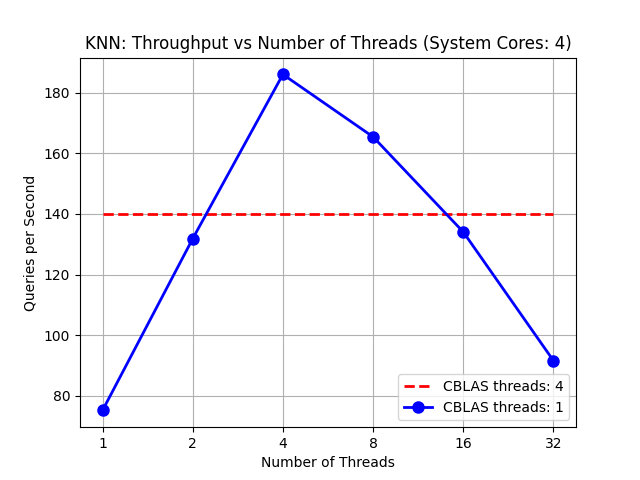
\includegraphics[width=1\linewidth]{figures/knn_throughput_vs_threads.png}
\caption{Performance comparison of different threading configurations for exact k-NN on the MNIST dataset.}
\label{fig:knn_throughput_vs_threads}
\end{figure}

\section{All-to-All Approximate Nearest Neighbors Solution}

In this section, we extend the parallelized k-NN framework to approximate all-to-all nearest neighbors (A2A-ANN), where the query set and candidate set coincide ($Q = C$). To ensure scalability on large datasets, we introduce approximation techniques based on clustering, which limit exhaustive comparisons while maintaining acceptable accuracy levels. This section elaborates on the clustering strategy, parallel workload distribution, memory management considerations, and the trade-off between approximation accuracy and computational throughput.

\subsection{Clustering Strategy: K-Means Partitioning}

To reduce the computational complexity of pairwise distance calculations, we partition the dataset into $K_c$ clusters using the k-means clustering algorithm. Each data point $x_i \in C$ is assigned to one of $K_c$ cluster centroids based on its minimum Euclidean distance. 

The k-means algorithm operates in two primary phases:
\begin{itemize}
    \item \textbf{Initialization:} Cluster centroids are initialized via random sampling to ensure a diverse 
    starting configuration. Data points not selected as initial centroids are assigned to the nearest centroid 
    based on Euclidean distance.
    
    \item \textbf{Cluster Merging:} After initial assignment, clusters with fewer than $K$ points are iteratively
    merged with their nearest neighboring cluster. The proximity between clusters is determined by the Euclidean 
    distance between their centroids, where each centroid is computed as the mean of the points assigned to the 
    respective cluster. This merging strategy ensures that all clusters have a sufficient number of points for 
    $K$-nearest neighbor computation while preserving local structure.
\end{itemize}

By restricting the nearest neighbor search to within clusters, we reduce the effective search space from $N$ points 
to approximately $N/K_c$ points per query.

This clustering stage serves as a coarse pre-filtering mechanism, significantly reducing the number of distance 
computations without major sacrifices in accuracy.

\subsection{Workload Balancing and Parallelization}

The all-to-all ANN implementation retains a multi-threaded design to achieve high computational throughput. 
However, unlike the $Q \neq C$ scenario where queries are evenly split among threads, the cluster-based strategy
introduces non-uniform workload distribution due to varying cluster sizes.

To address this, we employ a greedy load-balancing strategy:
\begin{itemize}
    \item Clusters are sorted in descending order based on the number of points.
    \item A bin-packing approach is used where each cluster is assigned to the thread with the currently 
    least assigned workload (in terms of total points).
    \item Each thread independently computes intra-cluster $K$ nearest neighbors, avoiding inter-thread 
    synchronization during the computation phase.
\end{itemize}

This dynamic allocation minimizes thread idling and balances the computational workload even when cluster 
sizes vary significantly. Parallel efficiency is maximized, and the linear scaling behavior with respect to 
CPU cores is largely retained, as demonstrated in the benchmarking results.

\subsection{Memory Efficiency Considerations}

The introduction of clustering contributes to memory savings by limiting the scope of pairwise distance 
calculations. Instead of allocating memory for a full $N \times N$ distance matrix, each thread only requires 
memory for:
\begin{itemize}
    \item The distance matrix corresponding to points within its assigned cluster(s), typically of size 
    $O\left(\left(\frac{N}{K_c}\right)^2\right)$.
    \item Temporary buffers for sorting and top-$K$ selection, scaled proportionally to cluster sizes.
    \item Precomputed norms of all points, shared across threads in a read-only fashion.
\end{itemize}

Memory buffers are pre-allocated and reused across multiple cluster batches, avoiding frequent allocations and 
reducing memory fragmentation. The maximum memory footprint is proportional to the largest cluster size and can
be bounded by adjusting $K_c$ accordingly.

This memory-aware design allows the algorithm to process datasets that would otherwise exceed the memory capacity 
in an exact all-to-all k-NN scenario.

\subsection{Accuracy and Throughput Trade-off}

The principal trade-off in the A2A-ANN approach arises from the choice of the number of clusters $K_c$, 
which directly impacts both computational throughput and approximation accuracy:
\begin{itemize}
    \item \textbf{High $K_c$ (many clusters):} Reduces the size of intra-cluster search, improving throughput 
    but potentially missing true nearest neighbors that reside in other clusters, thereby reducing recall.
    \item \textbf{Low $K_c$ (few clusters):} Increases the intra-cluster search space, reducing computational 
    gains but improving recall by capturing more candidate neighbors.
\end{itemize}

This trade-off is quantified in terms of:
\begin{itemize}
    \item \textbf{Neighbor Recall:} The proportion of true nearest neighbors retrieved by the approximate method compared to exact computation.
    \item \textbf{Throughput:} The number of queries processed per second, inversely proportional to runtime.
\end{itemize}

Figure~\ref{fig:ann_recall_vs_clusters} illustrates this trade-off on the MNIST dataset for different thread 
counts. The minor fluctuations in recall across different thread runs are due to the random initialization of 
cluster centroids. The results show that practical recall levels of around 90\% can be achieved while significantly 
reducing runtime. However, when the number of clusters exceeds 100, recall declines sharply, dropping below 60\%,
indicating that overly aggressive clustering can adversely impact accuracy.

\begin{figure}
    \centering
    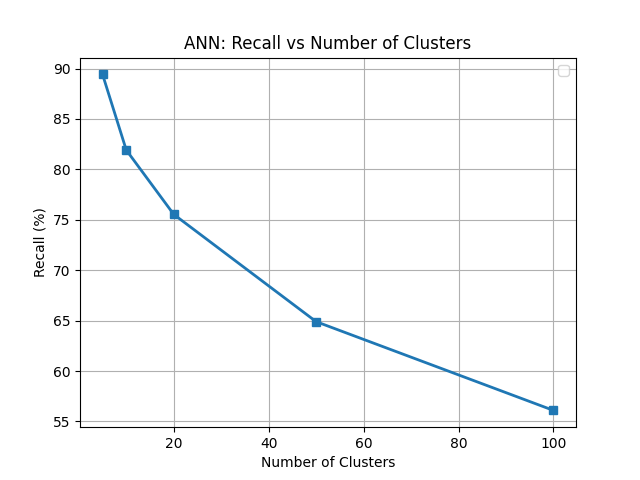
\includegraphics[width=1\linewidth]{figures/ann_recall_vs_clusters.png}
    \caption{Trade-off between recall and throughput for varying cluster counts ($K_c$) on the MNIST dataset.}
    \label{fig:ann_recall_vs_clusters}
\end{figure}

In summary, the clustering parameter $K_c$ provides an effective lever to tune the algorithm's behavior 
between accuracy and efficiency, allowing flexible adaptation to different deployment scenarios.

\subsection{Throughput Scaling with Threads and Clusters}

Figure~\ref{fig:ann_throughput_vs_threads} presents the throughput of the All-to-All Approximate Nearest 
Neighbors (A2A-ANN) implementation as a function of the number of application-level threads, for different 
numbers of clusters. Across all configurations, we observe a consistent trend: throughput increases with the 
number of threads up to the point where it matches the number of physical CPU cores. Beyond this point, further
increasing the number of threads leads to saturation or even slight performance degradation, primarily due to 
overheads from thread contention and context switching. This behavior highlights the importance of aligning the
number of threads with the available hardware parallelism for optimal performance.

In addition to threading, the figure also demonstrates the effect of clustering on throughput. As the number of
clusters increases, throughput improves across all thread counts. This improvement is attributed to the reduced 
computational cost of nearest neighbor searches within smaller clusters, as opposed to performing exhaustive 
comparisons across the entire dataset. The combined effect of parallelism and clustering results in significant 
acceleration, especially when both factors are tuned appropriately.

\begin{figure}
    \centering
    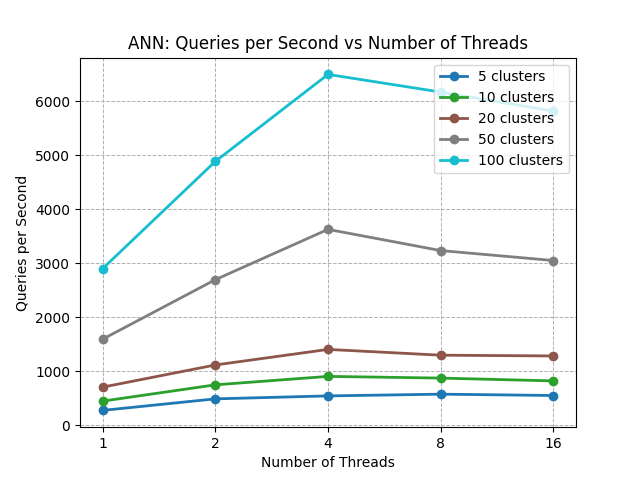
\includegraphics[width=1\linewidth]{figures/ann_throughput_vs_threads.png}
    \caption{Throughput vs number of threads over different number of clusters ($K_c$)}
    \label{fig:ann_throughput_vs_threads}
\end{figure}

\section{Conclusion and Future Work}

In this report, we presented a parallelized framework for exact k-NN and approximate all-to-all nearest 
neighbors (A2A-ANN) search. The solution effectively leverages multi-threading, efficient matrix computations, 
and clustering techniques to achieve high throughput and scalable performance on multi-core systems. Our results 
demonstrate that significant speedups can be obtained while maintaining acceptable recall levels by adjusting the 
number of clusters, with optimal performance observed when the number of threads matches the number of physical 
cores.

A key limitation of the current approach is that nearest neighbor candidates are restricted to within individual 
clusters, which can negatively impact recall at high cluster counts. As future work, we plan to address this by 
combining candidates from multiple neighboring clusters to improve accuracy. Additionally, we will investigate 
more advanced clustering strategies, including balanced clustering and hierarchical methods, to further enhance 
workload distribution and recall. Expanding the implementation to distributed environments and incorporating GPU
acceleration are also promising directions to handle even larger datasets and further reduce execution time.

\bibliographystyle{IEEEtran}
\bibliography{references}
\end{document}
